%!TEX encoding = UTF-8 Unicode
%!TEX root = ../compendium2.tex

\Assignment{photo}

\subsection{Bakgrund}
Detta projekt innebär att du ska implementera en egen bilbehandlingsapplikation, en mycket förenklad variant av \emph{Phtotoshop} eller \emph{Gimp}. 

En digital bild består av ett rutnät, en s.k. matris \Eng{matrix}, av pixlar, var och en med en viss färg. Om man har många små pixlar bredvid varandra i ett rutnät, så flyter de samman för ögat och betraktaren upplever en bild.

Bilder kan manipuleras genom applicering av olika s.k. \emph{filter}, som förändrar bildens pixlar på ett intressanta sätt. Du ska, utifrån given matematisk teori, implementera olika filter med hjälp av speciella matrisoperationer.


Det finns olika system för hur man färgsätter pixlar. T.ex. så används CMYK-systemet (cyan, magenta, gul, svart) vid blandning av färg som ska tryckas på papper eller annat material. På en dator, däremot, används vanligtvis RGB-systemet, som har de tre grundfärgerna röd, grön och blå. Mättnaden av varje grundfärg anges av ett heltal som vi i fortsättningen förutsätter ligger i intervallet [0, 255]. 0 anger ''ingen färg'' och 255 anger ''maximal färg''. Man kan därmed representera 256 × 256 × 256 = 16 777 216 olika färgnyanser. Man kan också representera gråskalor; det gör man med färger som har samma värde på alla tre 
grundfärgerna: (0, 0, 0) är helt svart, (255, 255, 255) är helt vitt. 

I detta projekt kommer vi skapa matriser av heltal för att beräkna intressanta egenskaper hos en bild, till exempel intensiteten för varje pixel. 
För att spara plats vid bearbetning av stora bilder så använder vi, heltalsmatriser med typen \code{Short}, som använder 16 bitar i minnet, i ståället för \code{Int}, som använder 64 bitar i minnet. 

\subsection{Förberedelser}

I detta projekt har du nytta av följande delar av \href{https://github.com/lunduniversity/introprog-scalalib}{\texttt{introprog-scalalib}} och \code{java.awt}:

\begin{itemize}
\item \code{introprog.Image} för bildhantering.
\item \code{introprog.PixelWindow} och \code{introprog.Dialog} för användarinteraktion.
\item \code{introprog.IO} för filhantering.
\item \code{java.awt.Color} för hantering av pixelfärger.
\end{itemize}
Läs noga dokumentationen för klasserna i introprog här och gör egna experiment i REPL så du förstår hur de kan användas: 
\url{https://cs.lth.se/pgk/api/}\\
Läs om klassen \code{java.awt.Color} här:\\\url{https://docs.oracle.com/en/java/javase/11/docs/api/java.desktop/java/awt/Color.html}
Hämta och studera noga den kod som är given för detta projekt här:\\
\url{https://github.com/lunduniversity/introprog/tree/master/workspace/}

\subsection{Matris med värden av typen \code{Short}}

\Task \textbf{\code{Matrix}}.
I den givna kodfilen \code{Matrix.scala} finns hjälp-funktioner för att skapa och uppdatera matriser med värden av typen \code{Short}, för att spara minne vid stora bilder.  

Gör klart saknade implementationer och testa noga i REPL så att allt fungerar som det ska innan du går vidare. \emph{Tips:} Du har nytta av \code{Array.tabulate}. 
\begin{REPLsmall}
scala> import photo.*

scala> val m = Matrix(3,3)(1,2,3,4,5,6,7,8,9) // en 3x3-matiris med Short-värden
val m: photo.Matrix = Array(Array(1, 4, 7), Array(2, 5, 8), Array(3, 6, 9))

scala> m(0,1)
val res0: Short = 4

scala> m(1,0) = 42

scala> m
val res1: photo.Matrix = Array(Array(1, 4, 7), Array(42, 5, 8), Array(3, 6, 9))

scala> m.row(0)
val res2: Array[Short] = Array(1, 42, 3)
\end{REPLsmall}

\subsection{Användargränssnitt}

När appen startar så visas ett fönster enligt fig. \ref{photo:fig:main-window}, implementerat av givna koden i \code{Main.scala}. Med hjälp av givna \code{Button.scala} skapas en kolumn med knappar som är klickbara. Studera koden i \code{Main.scala} och \code{Button.scala} noga så att du förstår vad som händer. Ännu öppnas inget ImageEditor-fönster, men det ingår i näst uppgift.

\begin{figure}[H]
\centering
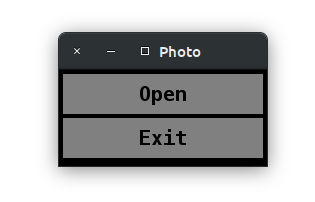
\includegraphics[width=0.4\textwidth]{../img/w12-assignment-photo/photo-main.png}
\caption{Photo-applikationens startfönster.}
\label{photo:fig:main-window}
\end{figure}

\Task \textbf{\code{ImageEditor}}. Följande krav ska implementeras: 

\begin{itemize}
\item Du ska skapa en kodfil \code{ImageEditor.scala} som innehåller en klass med samma namn som implementerar ett bildredigeringsfönster med en kolumn med knappar till vänster och en bild inläst från fil till höger, så som visas i fig. \ref{photo:fig:editor-one-filter}. 

\item Vid tryck på Exit-knappen ska en varningsfråga ''Ok to Exit without save?'' ges med \code{introprog.Dialog.isOK} och användaren ska kunna ångra avslut. Om avslut ändå väljs så ska detta ske med \code{System.exit(0)} så att alla ev. aktiva fönster och tillhörande trådar avbryts direkt.

\item Vid tryck på Open-knappen ska en fil väljas med hjälp av \code{introprog.Dialog.file}. Om det i aktuell katalog finns en underkatalog vid namn \code{images} så ska filbläddringen börja där, annars i aktuell katalog. 

\item Efter OK på filöppningen ska en bild öppnas i ett bildredigeringsfönster enligt fig. \ref{photo:fig:editor-one-filter} med knapparna Save, Undo, Close, plus en knapp för varje filter, till vänster om bilden. Fönstrets höjd och bredd ska avpassas så att hela bilden och alla knappar får plats.

\begin{figure}
\centering
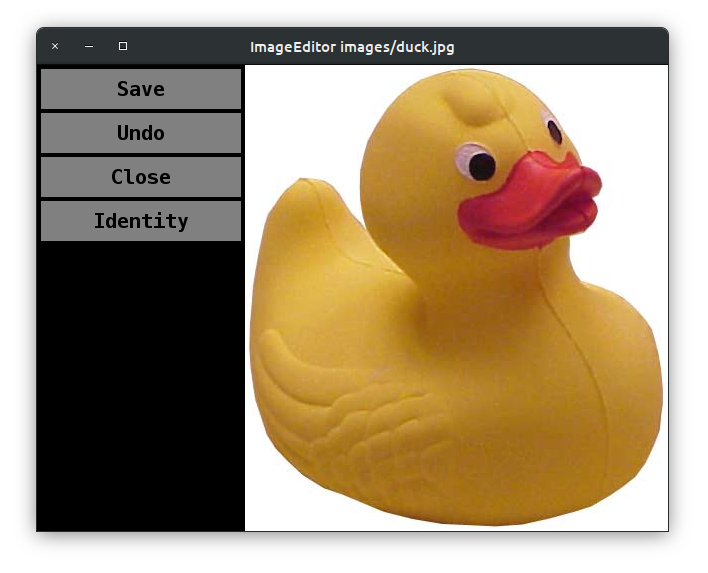
\includegraphics[width=0.8\textwidth]{../img/w12-assignment-photo/photo-duck.png}
\caption{Bildredigeringsfönstret, innan fler filter (utöver identitetsfiltret) implementerats. Varje filter som implementeras ska ha en motsvarande knapp.}
\label{photo:fig:editor-one-filter}
\end{figure}

\item Huvudfönstret och alla bildredigeringsfönster ska fungera parallellt. Detta ska du åstadkomma genom att händelseloopen i \code{ImageEditor}-klassen körs som argument till metoden \code{runInParallell} enligt nedan: 
\begin{CodeSmall}
  def runInParallell(block: => Unit) = 
    new Thread{ override def run(): Unit = block }.start

  def startEventLoop(): Unit = runInParallell:
    // initialisering och händelseloop här
\end{CodeSmall}

\item Det ska gå att göra Undo i flera steg och återställa alla bilder före applicering av filter i tur och ordning. \emph{Tips:} Inför i attributet \code{var history: Vector[Image]} som från början innehåller den ursprungliga bilden.

\item Fönstrets titel ska innehålla namnet \code{ImageEditor} och de två sista delarna av den sökväg \Eng{path} som öppnats, enligt exempel i fig. \ref{photo:fig:editor-one-filter}, eftersom en fullständig sökväg t.ex. \texttt{/home/userxyz/workspace/photo/images/duck.jpg} riskerar att inte få plats i fönstrets titelbalk.

\item Vid Save ska fråga om filnamn ställas med \code{introprog.Dialog.file} och kontroller göras om filen redan finns eller ej, och om den finns ska en fråga med \code{introprog.Dialog.isOK} ställas om den ska skrivas över eller ej.

\item Alla implementerade filter ska ha en knapp som applicerar filtret och sparar resultatet i historiken så att filtret kan ångras med Undo. Om filtret har argument så ska en informativ dialog öppnas där användaren kan ange argument via \code{introprog.Dialog.input}. Filterknapparna ska vara sorterade i bokstavsordning efter filtrets namn, se fig. \ref{photo:fig:photo-jay-sobel}.
\end{itemize}




\subsection{Filter}

Du ska bygga vidare på givna koden i \code{Filter.scala} som visas nedan. Du ska implementera och testa ett antal olika filter som ändrar bilder på intressanta sätt med hjälp av olika matrisalgoritmer.

\scalainputlisting[basicstyle=\ttfamily\fontsize{9.5}{11}\selectfont]{../workspace/w13_photo_proj/Filter.scala}

\noindent \code{Filter.scala} innehåller en bastyp för alla filter med ett antal medlemmar som alla filter ska implementera, enligt nedan krav. Det finns ett färdigimplementerat filter, \code{Identity}, som kan användas för testsyften; detta filter gör inget annat än kopierar alla bildpunkter till en ny bild och har således ingen editerande effekt.

\begin{itemize}
\item Metoden \code{apply} ska returnera en ny bilden där filtret applicerats, utan att förändra inparameter-bilden. 

\item Ett filter ska kunna ha noll eller flera argument av typen \code{Double} som kan påverka vad som händer när filtret appliceras. Varje sådant argument ska i tur och ordning ha en kort, instruktiv beskrivning i sekvensen \code{argDescription}.

\item Metoden \code{intensity} ska beräkna en s.k. \emph{intensitetsmatris} och behövs vid implementeringen av gråskale-, Gauss- och Sobel-filtren. Hur en intensitetsmatris beräknas beskrivs nedan. 

\item Metoden \code{convolve} ska göra en s.k. faltning (medelvärdesbildning i matriser) och behövs vid implementering av Gauss- och Sobel-filtren. Hur en faltning görs beskrivs nedan.

\item Alla implementerade filter ska finnas i sekvensen \code{byIndex}, som används i tabellen \code{byName}. Dessa behövs för att skapa alla filterknappar och applicera respektive filter.
\end{itemize}

\noindent Du ska implementera och testa alla filter i uppgifterna nedan, ett i taget. Uppgifterna är ordnade i stigande svårighetsgrad.

\begin{figure}
\centering
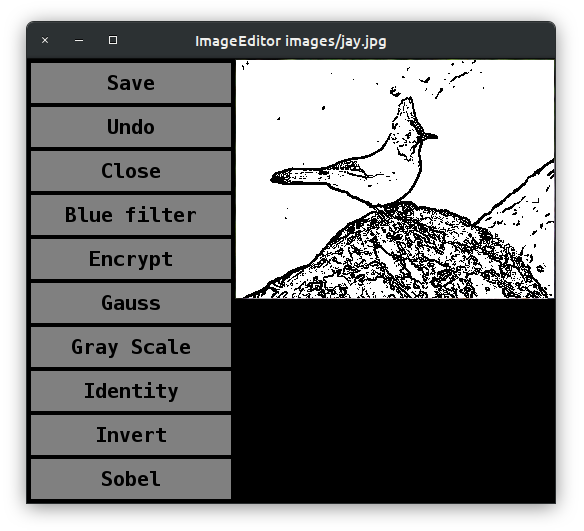
\includegraphics[width=0.8\textwidth]{../img/w12-assignment-photo/photo-jay-sobel.png}
\caption{Bildredigeringsfönstret med alla filter implementerade. Ett kontruförstärkande så kallat Sobel-filter är applicerat med tröskelvärde 150.}
\label{photo:fig:photo-jay-sobel}
\end{figure}


\Task \textbf{Blåfilter.} Skapa ett filter i ett singelobjekt med namn \code{Blue} som vid applicering ger en blå version av bilden, där varje pixel bara innehåller den blå komponenten. \emph{Tips:} Du har nytta av metoden \code{getBlue} i klassen \code{java.awt.Color}. 

\Task \textbf{Negativ.} Skapa ett filter \code{Invert} som inverterar en bild, dvs skapar en ''negativ'' kopia av bilden. Ljusa färger ska alltså bli mörka och mörka färger ska bli ljusa.
Fundera över vad som kan menas med en inverterad eller negativ kopia. \emph{Tips:} Även de nya RGB-värdena ska vara i heltal i intervallet 0 -- 255. De nya RGB-värdena beräknas \emph{inte} med något divisionsuttryck över de gamla värdena (då skulle de nya värdena bli decimaltal och inte heltal i intervallet 0 -- 255). 

\Task \textbf{Gråskalefilter.} Skapa ett filter \code{GrayScale} som gör om bilden till en gråskalebild. Implementera först \code{intensity}-metoden i \code{trait Filter} genom att bilda medelvärdet av alla tre RGB-komponenterna. Använd sedan intensiteten för varje pixel för att bestämma gråskalenivån. Om intensiteten i en pixel till exempel är 105 så ska den nya gråskale-pixeln var ett \code{Color}-objekt med RGB-värdena (105, 105, 105).

\Task \textbf{Kryptering.} Skapa ett filter \code{XOrCrypto} som krypterar bilden med xor-operatorn ˆ. Denna operator gör binär xor mellan bitarna i ett heltal. Exempelvis ger 8 ˆ 127 värdet 119. Om man gör xor igen med 127, alltså 119 ˆ 127, får man tillbaka värdet 8. Varje pixel krypteras genom att använda xor-operatorn med ursprungsvärdena för rött, grönt och blått tillsammans med slumpmässiga heltalsvärden som genereras ur en ny instans av \code{scala.util.Random}. Tre nya slumptal ska dras för varje pixels RGB-komponent ur samma Random-instans. Låt användaren ge ett argument som du använder som slumptalsfrö vid skapande av \code{Random}-instansen. På så sätt kan du återskapa bilden genom att applicera krypteringsfiltret igen, med samma argument, på den numera krypterade bilden.

Om filtrets \code{argDescriptions}-sekvens är icke-tom så ska \code{ImageEditor} fråga efter varje argument i tur och ordning och visa varje beskrivning i dialogrutan. Användarens indata görs om till ett decimaltal av typen \code{Double} före att argumenten används i metoden \code{apply}. Bestäm själv hur du vill hantera defaultvärden och felhantering om användaren anger en sträng som inte går att göra om till en \code{Double}. \emph{Tips:} Du har nytta av \code{toDoubleOption} och \code{getOrElse}.

\begin{CodeSmall}
  object XOrCrypto extends Filter:
    val name = "Encrypt"
    override val argDescriptions = Seq("Encryption key")

    def apply(im: Image, args: Double*): Image = ???
\end{CodeSmall}

\begin{REPLnonum}
scala> Seq(8, 127, 8 ^ 127).map(_.toBinaryString)
val res0: Seq[String] = List(1000, 1111111, 1110111)

scala> 8 ^ 127
val res1: Int = 119

scala> 119 ^ 127
val res2: Int = 8
\end{REPLnonum}

\begin{figure}
\centering
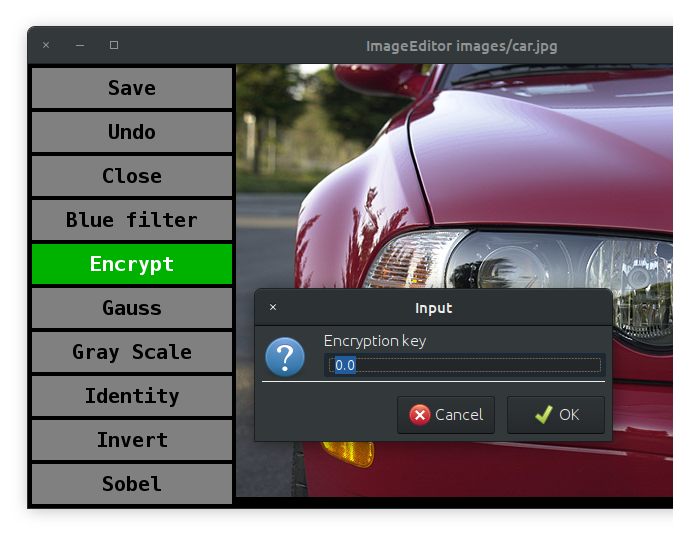
\includegraphics[width=0.85\textwidth]{../img/w12-assignment-photo/photo-xor.png}
\caption{Krypteringsfilter före applicering, under pågående inmatning av nyckel. }
\label{photo:fig:photo-xor}
\end{figure}
  

\Task \textbf{Gaussfilter.} Ett Gaussfilter gör bilden lite mindre skarp. Gaussfiltrering är ett exempel på så kallad \emph{faltningsfiltrering}. Faltning \Eng{convolution} är en slags lokal medelvärdesbildning. Nya pixlar skapas genom att kombinera varje pixel med dess omgivande pixlar enligt en speciell matrisalgoritm.

För att åstadkomma detta utnyttjar man en så kallad \emph{faltningskärna} K som är en liten kvadratisk heltalsmatris. Man placerar K över varje element i intensitetsmatrisen och multiplicerar varje element i K med motsvarande element i intensitetsmatrisen. Man summerar produkterna och dividerar summan med summan av elementen i K för att få det nya värdet på intensiteten i punkten (alltså ett slags medelvärde). Divisionen görs för att den nya intensiteten ska hamna i rätt intervall (0 -- 255).
Exempel:

\vspace{1em}
\begin{minipage}{5cm}
\begin{displaymath}
\mathit{intensity} = \left(
\begin{array}{ccccc}
5 & 4 & 2 & 8 & \ldots \\
4 & 3 & 4 & 9 & \ldots \\
9 & 8 & 7 & 7 & \ldots \\
8 & 6 & 6 & 5 & \ldots \\
\vdots & \vdots & \vdots & \vdots & \ddots
\end{array}
\right)
\end{displaymath}
\end{minipage}\hspace{2cm}
\begin{minipage}{5cm}
\begin{displaymath}
K = \left(
\begin{array}{ccc}
0 & 1 & 0 \\
1 & 4 & 1 \\
0 & 1 & 0
\end{array}
\right)
\end{displaymath}
\end{minipage}

\vspace{2em}\noindent Här är summan av elementen i $K$ $1+1+4+1+1 = 8$. För att räkna ut det nya värdet på intensiteten i punkten \code{(1, 1)} med det nuvarande värdet är 3, beräknar man följande:

\begin{displaymath}
\mathit{newintensity} = \frac{0 \cdot 5 + 1 \cdot 4 + 0 \cdot 2 + 1 \cdot 4 + 4 \cdot 3 + 1 \cdot 4 + 0 \cdot 9 + 1 \cdot 8 + 0 \cdot 7}{8} = \frac{32}{8} = 4
\end{displaymath}


\noindent Man fortsätter med att flytta K ett steg åt höger och beräknar på motsvarande sätt ett nytt värde för elementet med index \code{(1)(2)} (där det nuvarande värdet är 4 och det nya värdet blir 5). Därefter gör man på samma sätt för alla element utom för ”ramen” dvs elementen i matrisens ytterkanter.

Implementera och testa noga först metoden\\
\code{convolve(p: Matrix, x: Int, y: Int, kernel: Matrix, weight: Int): Short}\\ i \code{trait Filter} som alltså ska ge den normerade produktsumman av \code{kernel} och punkterna i närheten av \code{(x,y)} i matrisen \code{p} normerat med \code{weight}. \code{Tips:} Du har nytta av metoderna \code{round} och \code{toShort}.

\begin{REPLnonum}
scala> import photo.*

scala> val p = Matrix(4,4)(5,4,2,8,4,3,4,9,9,8,7,7,8,6,6,5)
val p: photo.Matrix = Array(Array(5, 4, 9, 8), Array(4, 3, 8, 6), Array(2, 4, 7, 6), Array(8, 9, 7, 5))

scala> val K = Matrix(3,3)(0,1,0,1,4,1,0,1,0)
val K: photo.Matrix = Array(Array(0, 1, 0), Array(1, 4, 1), Array(0, 1, 0))

scala> Filter.convolve(p, 1, 1, K, K.flatten.sum)
val res0: Short = 4
\end{REPLnonum}

Skapa därefter ett filter \code{Gauss} som gör en faltning med hjälp av \code{convolve} för varje färgkomponent separat. Gör på följande sätt:
\begin{enumerate}
	\item Bilda tre \code{short}-matriser och lagra pixlarnas red-, green- och blue-komponenter i matriserna.
	\item Utför faltningen av de tre komponenterna för varje element och uppdatera \code{result} med de uträknade värdena.
	\item Elementen i ramen behandlas inte, men i \code{result} måste också dessa element få värden. Enklast är att flytta över dessa element oförändrade från \code{im} till \code{result}. (Man kan också sätta dem till \code{Color.BLACK}, men då kommer den filtrerade bilden att se något mindre ut.)
\end{enumerate}

Använd \code{kernel} $K$ enligt ovan och låt \code{weight} vara summan av alla element i $K$. 

Det kan vara intressant att prova med andra värden än 4 i mitten av faltningsmatrisen. Med värdet 0 får man en större utjämning eftersom man då inte alls tar hänsyn till den aktuella pixelns värde. Låt användaren mata in argument för mittvärdet, mellan 0 och 50, och beskriv detta i \code{argDescriptions}. \footnote{Det kan ibland vara svårt att se någon skillnad mellan den Gauss-filtrerade bilden och originalbilden. Om man vill ha en riktigt suddig bild så måste man använda en större matris som faltningskärna. Prova gärna detta som extrauppgift. }


\Task  \textbf{Sobelfilter.} Sobelfiltrering är, precis som Gaussfiltrering, en typ av faltningsfiltrering. Med Sobelfiltrering får man dock motsatt effekt i jämförelse med Gaussfiltrering, dvs man förstärker konturer i en bild. I princip deriverar man bilden i x- och y-led och sammanställer resultatet.

\begin{figure}[H]
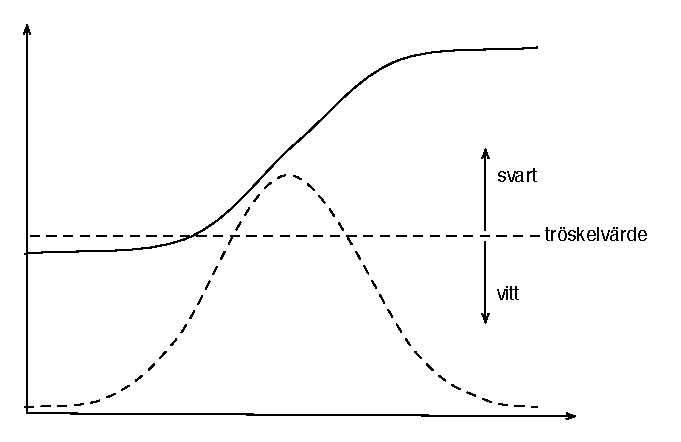
\includegraphics[width=0.9\textwidth]{../img/w12-assignment-photo/derivatabild2.pdf}
\caption { En funktion (heldragen linje) och dess derivata (streckad linje).}
\label{fig:photo:sobelfilter:derivatabild}
\end{figure}

I figur~\ref{fig:photo:sobelfilter:derivatabild} visas en funktion $f$ (heldragen linje) och funktionens derivata $f'$ (streckad linje). Vi ser att där funktionen gör ett ''hopp'' så får derivatan ett stort värde. Om funktionen representerar intensiteten hos pixlarna längs en linje i x-led eller y-led så motsvarar ''hoppen'' en kontur i bilden. Om man sedan bestämmer sig för att pixlar där derivatans värde överstiger ett visst tröskelvärde ska vara svarta och andra pixlar vita så får man en bild med starka konturer.

Nu är ju intensiteten hos pixlarna inte en kontinuerlig funktion som man kan derivera enligt vanliga matematiska regler. Men man kan approximera derivatan, till exempel med följande formel:

\begin{displaymath}
f'(x) \approx \frac{f(x+h) - f(x-h)}{2h}
\end{displaymath}

Om man låter $h$ gå mot noll så får man definitionen av derivatan.
Efter ytterligare teoretiska utredningar så kan man visa att det går att uttrycka derivering i en matris med hjälp av faltning enligt följande:
% 
% Uttryckt i Scala och matrisen \code{m: Matrix} så får man:

% \begin{Code}
% val derivative = (m(x, y + 1) - m(x, y-1)) / 2
% \end{Code}
\begin{enumerate}
	\item Beräkna intensitetsmatrisen med metoden \code{intensity}.
	\item För varje punkt i intensitetsmatrisen gör två faltningar med dessa kärnor:
$$
SobelX =
\begin{pmatrix}
  -1 & 0 & 1 \\
  -2 & 0 & 2 \\
  -1 & 0 & 1 \\
\end{pmatrix}
~\hspace{3em}~
SobelY =
\begin{pmatrix}
  -1 & -2 & -1 \\
  0 & 0 & 0 \\
  1 & 2 & 1 \\
\end{pmatrix}
$$
	Använd metoden \code{convolve} med vikten 1. Koefficienterna i matrisen $SobelX$ uttrycker derivering i x-led, medan $SobelY$ uttrycker derivering i y-led. För att förklara varför koefficienterna ibland är 1, ibland 2, ibland positiva och ibland negativa, måste man studera den bakomliggande teorin noggrant, men det gör vi inte här.
	\item Om resultaten av faltningen i en punkt betecknas med \code{sx} och \code{sy} så får man en indikator på närvaron av en kontur med \code{math.abs(sx) + math.abs(sy)}. Absolutbelopp behöver man eftersom man har negativa koefficienter i faltningsmatriserna.
	\item  Sätt pixeln till svart om indikatorn är större än tröskelvärdet, till vit annars. Låt tröskelvärdet bestämmas av ett argument som användaren kan ange.
\end{enumerate}
\noindent Skapa ett filter \code{Sobel} som implementerar konturförstärkning med ovan algoritm. Se exempel i fig. \ref{photo:fig:photo-jay-sobel}. Du ska låta användaren ge tröskelvärdet med argumentbeskrivningen \code{"Threshold (0.0 - 255.0)"}.


\Task Du ska inför redovisningen generera automatisk dokumentation baserat på dokumentationskommentarer enligt instruktioner i Appendix \ref{appendix:doc}. Du ska skriva relevanta dokumentationskommentarer för minst hälften av dina publika metoder. Det är ofta användbart att skriva dokumentationskommentarerna \emph{före} implementationen av metodkroppen.

\subsection{Frivilliga extrauppgifter}

\Task \textbf{Kortkommando}. Gör så att det blir möjligt att applicera filter med hjälp av tangentbordsinput. Utvidga \code{trait Filter} så att alla filter kan ha kortkommando. Skriv på knappen vad kortkommandot är så att användaren kan upptäcka det.

\Task \textbf{Kontrastfilter.} Om man applicerar kontrastfiltrering på en färgbild så kommer bilden att konverteras till en gråskalebild. (Man kan naturligtvis förbättra kontrasten i en färgbild och få en färgbild som resultat. Då behandlar man de tre färgkanalerna var för sig.) Många bilder lider av alltför låg kontrast. Det beror på att bilden inte utnyttjar hela det tillgängliga området 0–255 för intensiteten. Man får en bild med bättre kontrast om man ''töjer ut'' intervallet enligt följande formel (linjär interpolation):

\begin{Code}
val newIntensity = 255 * (intensity - 45) / (225 - 45)
\end{Code}

Som synes kommer en punkt med intensiteten 45 att få den nya intensiteten 0 och en punkt med intensiteten 225 att få den nya intensiteten 255. Mellanliggande punkter sprids ut jämnt över intervallet \code{[0, 255]}. För punkter med en intensitet mindre än 45 sätter man den nya intensiteten till 0, för punkter med en intensitet större än 225 sätter man den nya intensiteten till 255. Vi kallar intervallet där de flesta pixlarna finns för \code{[lowCut, highCut]}. De punkter som har intensitet mindre än \code{lowCut} sätter man till 0, de som har intensitet större än \code{highCut} sätter man till 255. För de övriga punkterna interpolerar man med formeln ovan (45 ersätts med \code{lowCut}, 225 med \code{highCut}).

Det återstår nu att hitta lämpliga värden på \code{lowCut} och \code{highCut}. Detta är inte något som kan göras enkelt, eftersom värdena beror på intensitetsfördelningen hos bildpunkterna. Man börjar därför med att först beräkna bildens intensitetshistogram, dvs hur många punkter i bilden som har intensiteten 0, hur många som har intensiteten 1, . . . , till och med 255.

I de flesta bildbehandlingsprogram kan man sedan titta på histogrammet och interaktivt bestämma värdena på \code{lowCut} och \code{highCut}. Så ska vi dock inte göra här. I stället bestämmer vi oss för ett procenttal \code{cutOff}, som användaren kan ange som argument från terminalen, och som  beräknar \code{lowCut} så att \code{cutOff} procent av punkterna i bilden har en intensitet som är mindre än \code{lowCut} och \code{highCut} så att \code{cutOff} procent av punkterna har en intensitet som är större än \code{highCut}.

\vspace{1em}

\noindent \textbf{Exempel}: antag att en bild innehåller 100 000 pixlar och att \code{cutOff} är 1.5. Beräkna bildens intensitetshistogram genom registrering av varje intensitet i en heltals-array \\  \code{val histogram = Array.ofDIm[Int](256)}\\och beräkna \code{lowCut} så att \\\code{histogram(0)} + \ldots + \code{histogram(lowCut)} = 0.015 * 100000 \\så nära det går att komma, det blir troligen inte exakt likhet. Beräkna \code{highCut} på liknande sätt.

\vspace{1em}


\noindent Sammanfattning av algoritmen:
\begin{enumerate}
	\item Beräkna intensitetsmatrisen.
	\item Beräkna bildens intensitetshistogram.
	\item Argument från användaren användas som \code{cutOff}.
	\item Beräkna \code{lowCut} och \code{highCut} enligt exempel ovan.
	\item Beräkna den nya intensiteten för varje pixel enligt interpolationsformeln och lagra de nya pixlarna i \code{result}.
\end{enumerate}
Skapa ett filter \code{Contrast} som implementerar algoritmen. I katalogen \emph{images} kan bilden \emph{moon.jpg} vara lämplig att testa, eftersom den har låg kontrast. Anmärkning: om \code{cutOff} sätts = 0 så får man samma resultat av denna filtrering som man får av \code{GrayScale}. Detta kan man se genom att studera interpolationsformeln.

\Task \textbf{Eget filter}. Skapa ett eget filter som utnyttjar att \code{apply}-metoden tar emot en sekvens av värden. Till exempel så kan du skicka in en array med fem värden där de två första värdena representerar ett intensitetsintervall och de tre sista värdena representerar röd-, grön- och blå-komponenterna till en färg som ska stoppas in där intensiteten hamnar utanför det givna intervallet. Ett annat alternativ kan vara att använda sig av metoder i \code{PixelWindow} för att välja specifika pixlar på originalbilden som sedan kan användas för att manipulera bilden i filtrets \code{apply}-metod. Valet är ditt!

\Task \textbf{Egna interaktiva verktyg}. Skapa valfria interaktiva redigeringsverktyg med mus- och tangentinput. Börja med ett markeringsverktyg som gör så att en rektangelformad del av bilden kan markeras med hjälp av musen. Gör det möjligt att applicera filter på den markerade delen av bilden. Du kan också göra så att argument till t.ex. Gauss-filtret kan ställas in med ett skjutreglage som du ritar under knappen och som kan regleras med mus eller piltangenter.
